\chapter{Introduction}

In this chapter I'll introduce some core concepts that are necessary to understand the following thesis. From machine learning and deep learning, to convolutions, autoencoders and deep clustering.  

\section{Machine learning and deep learning}

A machine learning algorithm is an algorithm that is able to learn from data. For this reason, machine learning allows us to tackle tasks that are too difficult to solve with fixed programs written and designed by human beings.

Machine learning tasks are usually described in terms of how the machine learning system should process an example. An example is a collection of features that have been quantitatively measured from some object or event that we want the machine learning system to process. In our case, the example is an image. The features of an image are usually the values of the pixels in the image.

One particular task related to images that interests us is classification. In this type of task, the computer program is asked to specify which of k categories some input belongs to. To solve this task, the learning algorithm is usually asked to produce a function $f: \mathbf{R}^n \rightarrow \{1, ..., k\}$. When
$y = f(x)$, the model assigns an input described by vector x to a category identified by numeric code $y$.

In order to evaluate the abilities of a machine learning algorithm, we must design a quantitative measure of its performance. Usually this performance measure is specific to the task being carried out by the system. For tasks such as classification,we often measure the accuracy of the model. Accuracy is just the proportion of examples for which the model produces the correct output.

Usually we are interested in how well the machine learning algorithm performs on data that it has not seen before, since this determines how well it will work when deployed in the real world. We therefore evaluate these performance measures using a test set of data that is separate from the data used for training the machine learning system.

Machine learning algorithms can be broadly categorized as \textit{unsupervised} or \textit{supervised}. Supervised learning algorithms experience a dataset containing features, but each example is also associated with a label or target. Unsupervised learning algorithms experience a dataset containing many features, then learn useful properties of the structure of this dataset. 

In the context of deep learning, we usually want to learn the entire probability distribution that generated a dataset. We are interested in unsupervised learning algorithms that perform other roles, like \textit{clustering}, which consists of dividing the dataset into clusters of similar examples.

Roughly speaking, unsupervised learning involves observing several examples of a random vector x, and attempting to implicitly or explicitly learn the probability distribution $\rho(x)$, or some interesting properties of that distribution.

Deep learning is a subset of machine learning. Deep feedforward networks, also often called feedforward neural networks,
or multilayer perceptrons (MLPs), are the quintessential deep learning models. The goal of a feedforward network is to approximate some function $f^*$. For example, for a classifier, $y = f^∗(x)$ maps an input $x$ to a category $y$. A feedforward network defines a mapping $y=f(x; \theta)$ and learns the value of the parameters $\theta$ that result in the best function approximation. 

Feedforward neural networks are called networks because they are typically represented by composing together many different functions. For example, we might have three functions $f(1)$ , $f(2)$ , and $f(3)$ connected in a chain, to form $f(x)=f(3) (f(2)(f(1)(x)))$. These chain structures are the most commonly used structures of neural networks. In this case, $f(1)$ is called the first layer of the network, $f(2)$ is called the second layer, and so on. The overall length of the chain gives the depth of the model. It is from this terminology that the name “deep learning” arises. The final layer of a feedforward network is called the output layer. During neural network training, we drive $f(x)$ to match $f^∗(x)$.

The training data provides us with noisy, approximate examples of $f^∗(x)$ evaluated at different training points. Each example $x$ is accompanied by a label $y\approx f^∗(x)$. The training examples specify directly what the output layer must do at each point $x$; it must produce a value that is close to $y$. The behavior of the other layers is not directly specified by the training data. The learning algorithm must decide how to use those layers to produce the desired output, but the training data does not say what each individual layer should do. Instead, the learning algorithm must decide how to use these layers to best implement an approximation of $f^*$. Because the training data does not show the desired output for each of these layers, these layers are called hidden layers.

Finally, these networks are called neural because they are loosely inspired by neuroscience.

\section{Convolutional neural networks and autoencoders}

\subsection{Convolutions and convolutional neural networks}

Convolutional networks \cite{6795724}, also known as convolutional neural networks or CNNs, are a specialized kind of neural network for processing data that has a known, grid-like topology. Examples include image data,
which can be thought of as a 2D grid of pixels. The name “convolutional neural network” indicates that the network employs the mathematical operation convolution \ref{eq:conv}. Convolutional networks are simply neural networks that use convolution in place of general matrix multiplication in at least one of their layers.
\begin{equation}\label{eq:conv}
    s(t) = \int x(a)w(t-a)da
\end{equation}
In convolutional network terminology, the first argument (in Equation \ref{eq:conv}, the function $x$) to the convolution is often referred to as the input and the second argument (in Equation \ref{eq:conv}, the function $w$) as the kernel. The output is sometimes referred to as the feature map.

Discrete convolution can be viewed as multiplication by a matrix. An example of 2D discrete convolutions can be seen in the Figure \ref{fig:conv}. 

\begin{figure}[h!]
    \centering
    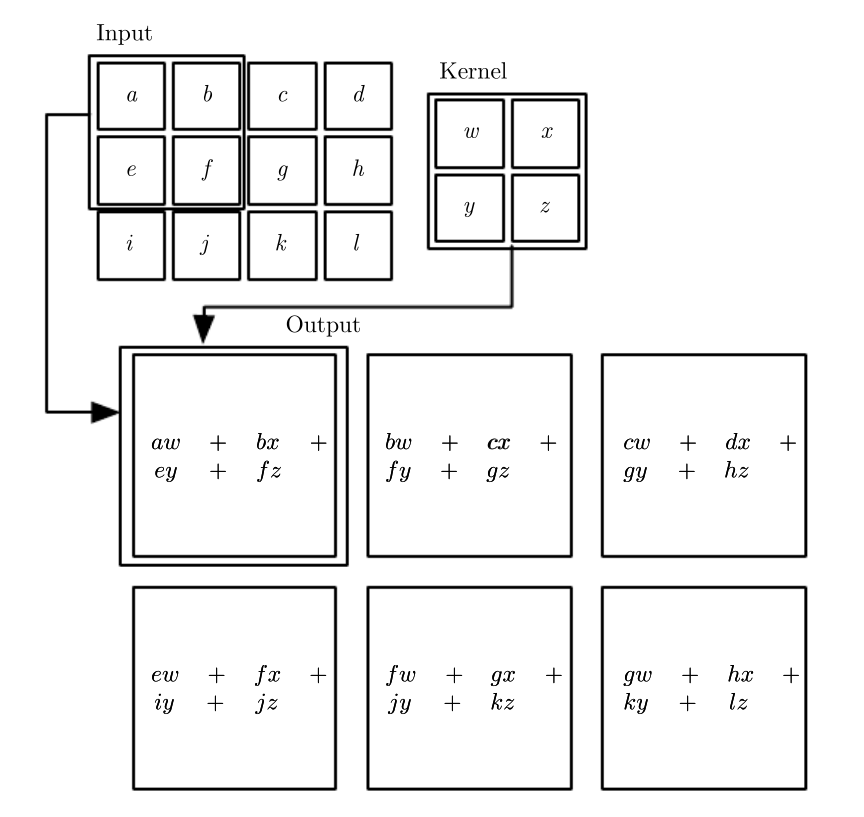
\includegraphics[width=10cm]{images/conv2D.png}
    \caption{Example of 2D convolutions.}
    \label{fig:conv}
\end{figure}

\subsection{Autoencoders}

An autoencoder is a neural network that is trained to attempt to copy its input to its output. Internally, it has a hidden layer $h$, also called embedded layer, that describes a code used to represent the input. The network may be viewed as consisting of two parts: an encoder function $h=f(x)$ and a decoder that produces a reconstruction $r=g(h)$.

If an autoencoder succeeds in simply learning to set $g(f(x))=x$ everywhere, then it is not especially useful. Instead,
autoencoders are designed to be unable to learn to copy perfectly. Usually they are restricted in ways that allow them to copy only approximately, and to copy only input that resembles the training data. Because the model is forced to prioritize which aspects of the input should be copied, it often learns useful properties of the data.

Our model is a convolutional autoencoder, meaning that it follows the structure of an autoencoder (encoder, embedded, decoder) where almost all layers are convolutional layers.

\section{Deep clustering}

Deep clustering algorithms can be broken down into three essential components: deep neural network, network loss, and clustering loss.

The deep neural network is the representation learning component of deep clustering algorithms. They are employed to learn low dimensional non-linear data representations from the dataset. Most widely used architectures are autoencoder based (mostly convolutional). 

The objective functions of deep clustering algorithms are generally a linear combination of an unsupervised representation learning loss, here referred to as network loss $L_r$ and a clustering oriented loss $L_c$. The total loss is formulated as
\begin{equation}
    L = L_r + \gamma L_c
\end{equation}
where $\gamma > 0$ controls the clustering loss. The neural network loss refer to the reconstruction loss of the autoencoder. Some models like DEC \cite{xie2016unsupervised} discard the network loss altogether in favour of just using clustering loss to guide both representation learning and clustering.

In deep clustering literature, we see the regular use of the following two evaluation metrics:

\begin{itemize}
    \item \textbf{Unsupervised Clustering Accuracy (ACC)}. \\ ACC is the unsupervised equivalent of classification accuracy. ACC differs from the usual accuracy metric since it uses a mapping function $m$ to find the best mapping between the cluster assignment output $c$ of the algorithm with the ground truth $y$. This mapping is required because an unsupervised algorithm may use a different label than the actual ground truth label to represent the same cluster. In particular, the unsupervised clustering accuracy is defined as
        \begin{equation}
            ACC = \max_m \frac{\sum_{i=1}^n \textbf{1}\{y_i=m(c_i)\}}{n}
        \end{equation}
        where $l_i$ is the ground-truth label, $c_i$ is the cluster assignment produced by the algorithm, and $m$ ranges over all possible one-to-one mapping between clusters and labels.
    
    \item \textbf{Normalized Mutual Information (NMI)}. \\
    NMI is an information theoretic metric that measures the mutual information between the cluster assignments and the ground truth labels. It is normalized by the average of entropy of both ground labels and the cluster assignments. It's defined as
    \begin{equation}
        NMI(Y,C) = \frac{2 \times I(Y;C)}{H(Y) + H(C)}
    \end{equation}
    where $Y$ are the class labels, $C$ are the cluster labels, $H$ is the entropy and $I(Y;C)$ is the mutual information between $Y$ and $C$.
\end{itemize}


\section{Applications in medical physics and previous works}

As one of the most popular approaches in artificial intelligence, deep learning has attracted a lot of attention in the medical physics field over the past few years. Embracing the current big data era, medical physicists equipped with these state-of-the-art tools aim to solve pressing problems in modern radiology. 

An example of this is Idiopathic pulmonary fibrosis (IPF), as one the most common type of pulmonary fibrosis. Machine learning and deep learning techniques are applied to High Resolution Computed Tomography (HRCT) for essentially two purposes. The first is to aid the radiologist in the diagnosis of the IPF. This is because the IPF has a specific texture pattern of the lung parenchyma (pattern UIP) that often is very similar to the texture pattern of other interstitial lung tissue diseases. When the diagnosis through images is not certain then it is necessary to resort to a biopsy, which is very invasive for the patient. Some works, like \cite{computerhtrc}, use ML techniques to analyse the HRCT images of interstitial lung diseases to automatically classify the IPF patterns. 

A second objective for the application of machine learning is the staging and prognosis of the IPF. Normally this step is done by functional tests, like a spirometry test. \cite{asd} tried to created a clinic/radiology model for staging and prognosis that includes parameters extracted from HRCT images. Most of the effort for staging and prognosis is concentrated on semantic segmentation of the lung tissue. The goal is to segment different patterns and feeding feature extracted from these patterns to a machine learning model. Most recently, the semantic segmentation is done by CNN models like \cite{8325482}. Also, \cite{WALSH2018837} uses a CNN directly for classification.

Our work falls into the second group where we try to approach in an unsupervised way the staging and prognosis of IPF utilising CNN to extract deep radiomics features from HRCT.